\documentclass[12pt]{article}

\usepackage{graphicx}
\usepackage{amsmath}
\usepackage{amssymb}
\usepackage{natbib}
\usepackage{amsfonts}
\usepackage{multicol}
\usepackage{float}
\usepackage{oldgerm}
\usepackage{bm}
\usepackage{mathtools}
\usepackage{wrapfig}
\usepackage{fancyhdr}
\usepackage[export]{adjustbox}
\usepackage{xcolor}
\usepackage[shortlabels]{enumitem}

\pagestyle{empty}

\setlength{\headsep}{0.5cm}
\setlength{\oddsidemargin}{-0.5cm}
\setlength{\textwidth}{16.5cm}
\setlength{\textheight}{24cm}
\voffset = -2cm


\pagestyle{fancy}
\fancyhf{}
\rfoot{
\includegraphics[width=1.0in]{cnm.png}}
\lfoot{Homework 6}
\setlength\parindent{0pt}
\begin{document}

\begin{center}
\hfil
{\large\bf {ENGR 2910-101: Circuit Analysis}}
\hfill Instructor: Brian Rashap\\
Homework 6:  \hfill Due: See Brightspace\\
\hrulefill\\
\end{center}

{\bf Question 1} [4] % P5-04

Assume the Op Amp below is ideal

\begin{figure}[h!]
\begin{center}
 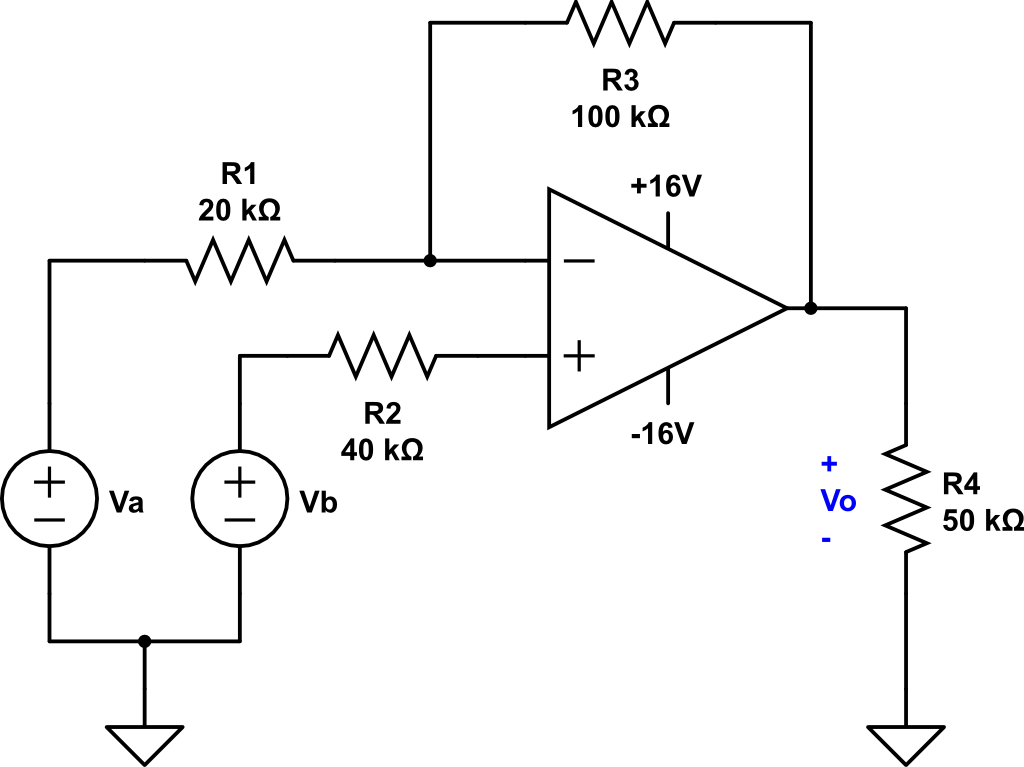
\includegraphics[scale=0.4]{p5_4.png}
\end{center}
\end{figure}

\begin{enumerate}[(a)]
\item Calculate $v_o$ if $v_a = 4V$ and $v_b = 0V$.
\item Calculate $v_o$ if $v_a = 2V$ and $v_b = 0V$.
\item Calculate $v_o$ if $v_a = 2V$ and $v_b = 1V$.
\item Calculate $v_o$ if $v_a = 1V$ and $v_b = 2V$.
\item If $v_0 = 1.6V$, specify the range of $v_a$ such that the amplifier does not saturate.
\end{enumerate}


\vspace{0.1in}

{\bf Question 2} [4] %P5-09

\begin{enumerate}[(a)]
\item Design an inverting amplifier with a gain of 4. Use an ideal ops amp, a $30 k \Omega$ resistor in the feedback path, and $\pm 12V$ power supplies. 
\item Using your design from part (a), determine the range of input voltages that will keep the op amp in the linear operating regions.  
\item Suppose you wish to amplify a $2V$ signal, using your design from part (a) with a variable feedback resistor. What is the largest value for the feedback resistance that keeps the op amp in the linear operating region? Using this resistance value, what is the new gain of the inverting amplifier. 
\end{enumerate}

\newpage

{\bf Question 3 [4]} % P5-16

Consider the ideal op amp below:

\begin{figure}[h!]
\begin{center}
 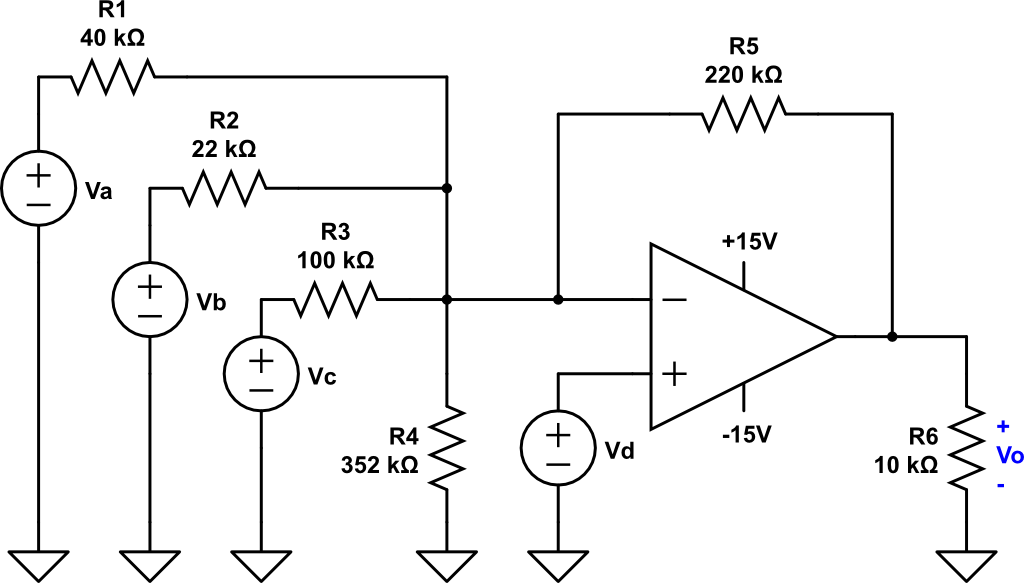
\includegraphics[scale=0.4]{p5_16.png}
\end{center}
\end{figure}

\begin{enumerate}[(a)]
\item Find $v_o$, if $v_a = 4V$, $v_b = 9V$, $v_c = 13V$, and $v_d = 8V$.
\item Assume $v_b$, $v_c$, and $v_d$ retain their values from part (a). Specify the range of $v_a$ such that the op amp operates in within the linear region.
\end{enumerate}

{\bf Question 4} [4] % P5-26

The resistor $R_f$ in the circuit below is adjusted until the ideal op amp saturates. Specify $R_f$ in kilohms.

\begin{figure}[h!]
\begin{center}
 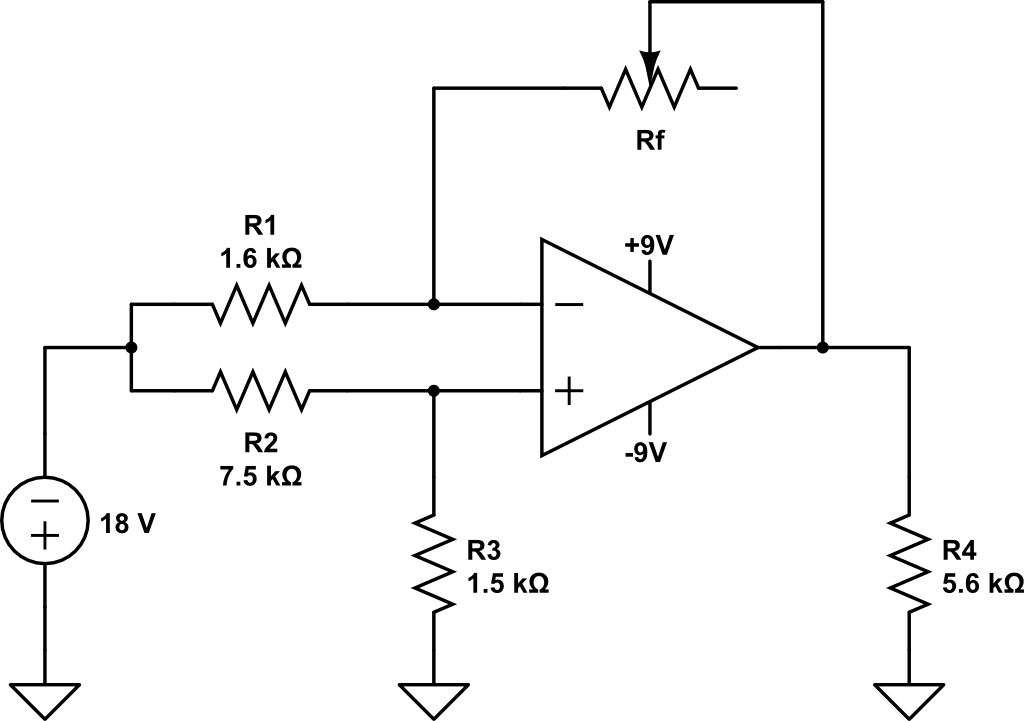
\includegraphics[scale=0.4]{p5_26.png}
\end{center}
\end{figure}

\newpage

{\bf Question 5} [4] % P5-32

In the differential amplifier shown below, find:

\begin{figure}[h!]
\begin{center}
 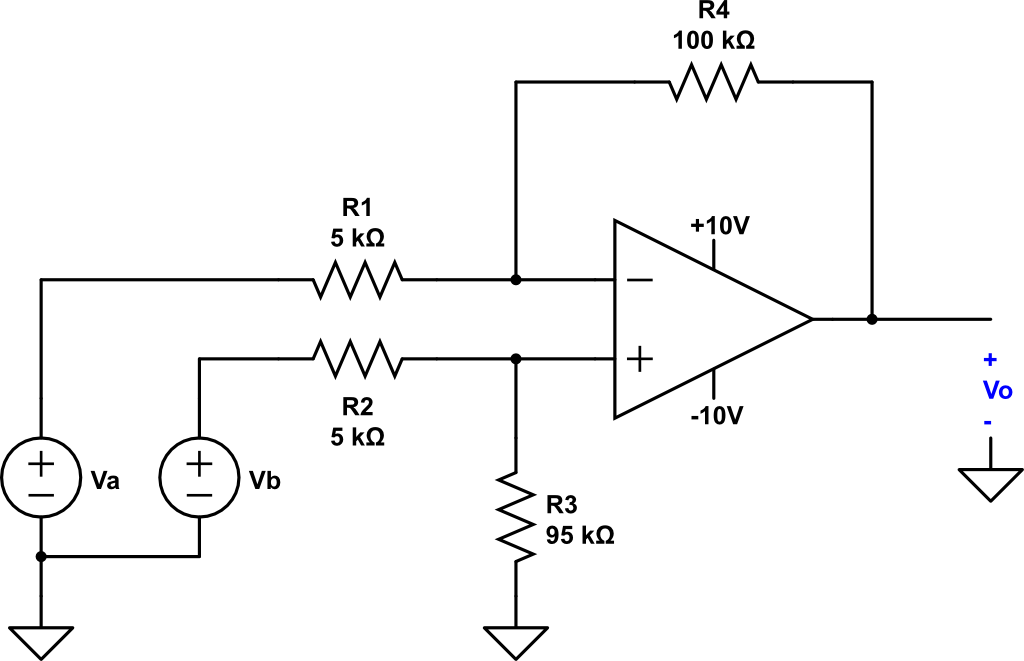
\includegraphics[scale=0.4]{p5_32.png}
\end{center}
\end{figure}

\begin{enumerate}[(a)]
\item The differential mode gain
\item The common mode gain
\item the CMRR
\end{enumerate}


\end{document}
